En \'este cap\'itulo se describir\'a al an\'alisis realizado para identificar los procesos llevados a cabo dentro de la cl\'inica, los problemas de la misma, sus causas y propuestas para solucionarlo

%--------------------------------------------------
\section{Contexto del sistema}

	La cl\'inica m\'edica de homeopat\'ia requiere de un sistema que realice las funciones que se realizan dentro de ella, y lleve el control de las citas por internet, llevar control sobre inventarios en farmacia as\' como los expedientes m\'edicos, con el fin de garantizar un mejor servicio a los pacientes de dicha cl\'inica.
La cl\'inica cuenta con 12 consultorios y una farmacia. Para que una consulta sea llevada a cabo, es necesario
que exista una cita previa, ya sea para Consulta General o Especialidad, la \'unica diferencia entre ambas es el costo y el docotr que atienda la consulta.
Para obtener una cita m\'edica es necesario llamar al tel\'efono de la cl\'inica, acudir personalmente a la misma, o bien, realizarla a trav\'es del sitio web de la cl\'inica. En caso de que no haya cupo en el horario que el usuario desee en ning\'un consultorio, se lo notificar\'a para que escoja un nuevo horario y/o fecha. Despu\'es de realizar la cita, el usuario recibir\'a u n\'umero de folio, con el cual deber\'a pagar en la caja de la cl\'inica a m\'as tardar diez minutos antes de la cita programada. En caso de que la cita no sea pagada en \'este tiempo, uno de los pacientes de espera podr\'a ingresar a esa consulta.
Al finaliza una consulta, el paciente recibir\'a una receta, la cual, en caso de querer abastecerla en la cl\'inica misma, deber\'a ir al m\'odulo de Farmacia para tomar un recibo de pago, pagar la cantidad indicada en el recibo en la caja, devolver el recibo con sello de "`Pagado"', y finalmente recoger sus medicamentos y su receta con sello de "`Entregado"'.

%--------------------------------------------------
\section{Procesos actuales}
\begin{itemize}
\item \bfseries{Registro de consulta m\'edica} \mdseries{: El paciente acude a la recepci\'on para solicitar una cita m\'edica para una fecha y horario especificados. La recepcionista revisa en su cuaderno de citas si no hay ninguna cita registrada para esa fecha y horario. En caso de que no haya ning\'un registro, lo anotar\'a en el cuaderno de citas y le indica al paciente que realice su pago en caja, y regrese a recepci\'on con un ticket de pago para poder registrar la cita como pagada.}
\item \bfseries{Pago de consulta m\'edica} \mdseries{: El paciente acude a caja pagando el monto correspodiente a una cita m\'edica y finalmente recibe un ticket de pago}
\item \bfseries{Pago de medicamentos} \mdseries{: El paciente acude a la farmacia con una receta m\'edica. El dependiente de la farmacia la revisa, verifica que en el almac\'en haya los suficientes medicamentos para abastecer la receta. En caso de que sí haya suficientes medicamentos, el dependiente procede a cobrarle al paciente el monto correspondiente a la receta m\'edica y finalmente el paciente recibe los medicamentos solicitados.}
\item \bfseries{Suministro de medicamentos} \mdseries{: El proveedor suministra medicamentos al almac\'en de la farmacia, y registra cada uno de los cambios que hizo en el stock en un cuaderno. Realiza \'este procedimiento cada quince d\'ias.}
\item \bfseries{Generaci\'on de expediente} \mdseries{: Cuando el expediente m\'edico de un paciente no existe, \'este debe ser generado. El m\'edico llena un formulario f\'isico con base en la informaci\'on que el paciente le proporciona. Al finalizar, \'este expediente es almacenado en un estante de archivos, intentando que el orden alfab\'etico (por apellido paterno) de los archivos no se altere.}
\item \bfseries{Cosulta} \mdseries{: Si el paciente pag\'o su consulta a tiempo, entrar\'a al consultorio que le haya sido asignado, y lo atender\'a el doctor que se halle en ese consultorio. La consulta no tiene una duraci\'on definida.}
\item \bfseries{Expedici\'on de receta m\'edica} \mdseries{: Al finalizar una consulta, si es necesario el doctor le otorgar\'a una receta m\'edica al paciente. \'Esto lo hace llenando un formulario (previamente impreso) donde indica los medicamentos recetados, su cantidad, el nombre del doctor y su firma o sello}
\end{itemize}
% - - - - - - - - - - - - - - - - - - - - - - - - -
\subsection{Participantes}

\begin{itemize}
\item \bfseries{M\'edico} \mdseries{.- Es el profesional autorizado legalmente para ejercer la medicina, y es el encargado de dar las consultas m\'edicas en la cl\'inica.}
\item \bfseries{Recepcionista} \mdseries{.- Es una persona asignada al \'area de "`Recepci\'on"'. Su trabajo es dar acceso a los pacientes al consultorio que indique la cita m\'edica que el paciente realiz\'o, o a los pacientes de espera . Tambi\'en se encarga de atender a los pacientes que deseen realizar citas m\'edicas via telef\'onica. }
\item \bfseries{Dependiente} \mdseries{.- Es la persona que atiende la farmacia. Se encarga de abastecer las recetas m\'edicas, y realizar el cobro correspondiente a las mismas.}
\item \bfseries{Cajero} \mdseries{.- Es la persona que atiende el m\'odulo de caja. Se encarga de recibir pagos de consultas m\'edicas y de entregar tickets de pago para verificar que el cliente pag\'o una consulta m\'edica.}
\item \bfseries{Paciente} \mdseries{.- Es la persona interesada en recibir una consulta. Acude a la recepci\'on de la cl\'inica para agendar una cita, y regresa el d\'ia de la cita para pagarla y tomar su consulta. Si lo necesita, acude a la farmacia con una receta m\'edica para comprar medicamentos}
\end{itemize}

% - - - - - - - - - - - - - - - - - - - - - - - - -
\subsection{Procesos}
\\ 
En la siguiente imagen (Figura 1.1) se muestra el funcionamiento de la Cl\'inica antes de que se implemente el sistema, en el c\'ual se puede apreciar de manera gr\'afica, que la cl\'inica tiene diversos problemas para poder organizar tanto la farmacia y la gesti\'on de citas, de igual manera no se puede determinar la salida o entrada tanto de dinero como de personas que adquieron una cita, determinando finalmente que el sistema que actualmente se utiliza es lento y deficiente, lo que a futuro puede provocar perdidas.
\begin{figure}[htbp!]
\centering
		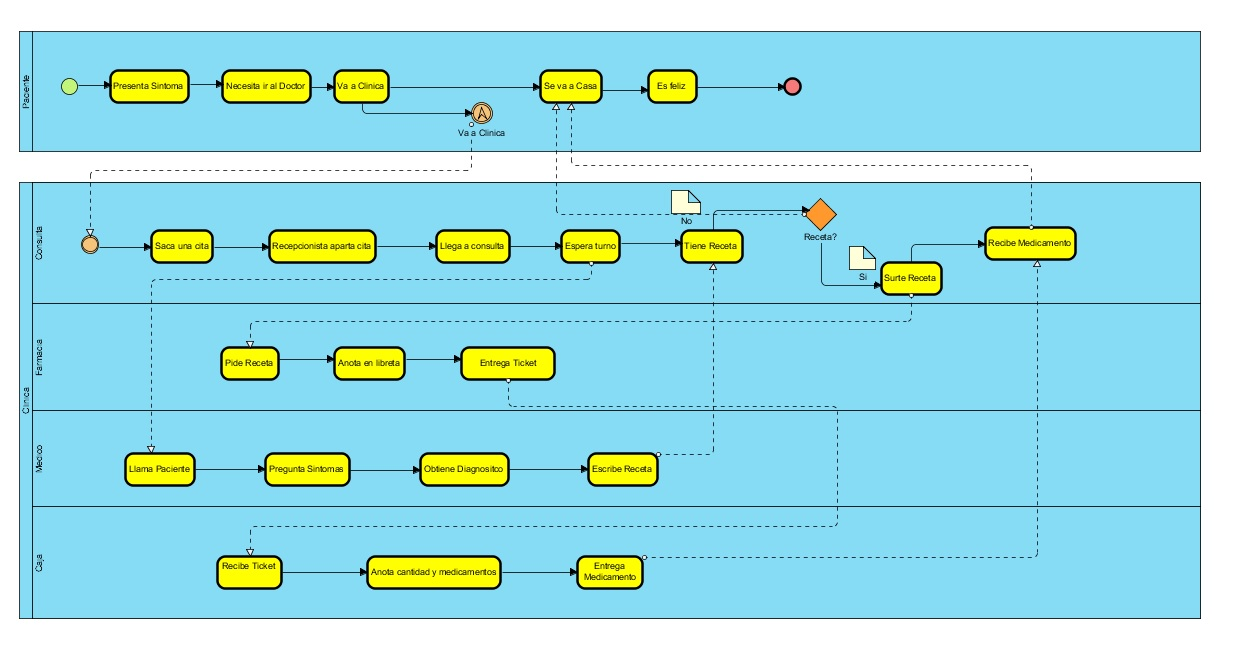
\includegraphics[width=.75\textwidth]{images/bpm1}
		\caption{Figura 2.1 Diagrama BPMN (Antes de Implementar el Sistema)}
	\end{figure}
\newpage
	
%--------------------------------------------------
\section{Problemas identificados}

% - - - - - - - - - - - - - - - - - - - - - - - - -
\subsection{Problema general}

No hay una forma efectiva, accesible y segura para llevar a cabo los procesos realizados dentro de la cl\'inica y para manipular la informaci\'on que se utiliza dentro de ella (expedientes m\'edicos, citas m\'edicas, pagos). 

% - - - - - - - - - - - - - - - - - - - - - - - - -
\subsection{Descomposición del problema}

\begin{enumerate}
\item Es tardado buscar un registro de cita en el cuaderno de registros.
\item A veces el encargado del cuaderno de registros olvida anotar otros registros.
\item En ocasiones el paciente no tiene la disponibilidad para acudir a la cl\'inica a agendar una cita.
\item No hay una forma definida para atender a los pacientes de espera.
\item No hay forma de registrar las transacciones hechas en la caja ni de controlar las salidas/entradas de dinero de la caja.
\item El proceso de compra de medicamentos es tardado, pues el dependiente debe revisar f\'isicamente si hay medicamentos suficientes para abastecer una receta.
\item Buscar un expediente m\'edico es tardado.
\item El c\'alculo del precio para una receta, lo realiza el dependiente, lo cual es tardado.
\item No hay una forma para mantener el control sobre el stock de medicamentos en el almac\'en
\item Para buscar un medicamento mediante una sustancia activa, el dependiente deber\'a leer los ingredientes activos de varios medicamentos hasta encontrar el que busca, lo cual es algo muy tardado, a menos de que el dependiente tenga mucha experiencia,.
\item No hay una forma definida para crear expedientes m\'edicos.
\item No hay una forma definida para vender medicamentos no controlados (sin receta m\'edica).
\item El flujo del dinero se realiza en dos lugares: en la caja (para pagar consultas) y en la farmacia (para vender medicamentos).
\item El sistema que actualmente usa la clinica es de analisis lento cuando se refiere a verificar cantidad de dinero y medicamentos que entraron o salieron de la clinica.%Comente este (diana)
\item Ya que la b\'usqueda de un expediente m\'edico es lenta, la modificaci\'on de estos es de igual manera lenta y no es eficaz, ya que todo el proceso es manual. %Checa si esta bien este problema (Diana)
\item Un paciente no tiene forma de saber la hora exacta de su consulta. Tiene qu\'e esperar hasta que el doctor pueda atenderlo.
\item El almacenamiento de expedientes m\'edicos es inseguro, pues cualquiera que tenga acceso a ellos puede modificarlos o extraerlos.
\item El almacenar una libreta de registros cada vez que se acaba representa una p\'erdida de recursos y espacio f\'isico.

\end{enumerate}

% - - - - - - - - - - - - - - - - - - - - - - - - -
\subsection{Análisis de causas}

\begin{figure}[htbp!]
		\includegraphics[width=1\textwidth]{images/ishikawa_consultas}
		\caption{Diagrama de Ishikawa}
	\end{figure}
\begin{enumerate}
\item Equipo:
\begin{itemize}
\item No generan nueva tecnología: Al faltar una nueva tecnología se quedan expuestos al almacenamiento masivo de información y optimización de sus tareas.
\item No se tiene equipo especializado a la tarea: No hay un equipo especializado para unir y sincronizar al mismo tiempo todas las tareas.
\end{itemize}
\item Materiales:
\begin{itemize}
\item No transportable: Los registros no son transportables debido a la perdida de los mismos y perder la organización.
\item Fácil de perder: Los archivos son destinados a perderse al no tener un control estricto de los mismo
\item Difíciles de almacenar: Los archivos que se juntan día a día crean almacenes enormes.
\item Sobre carga de archivos(papeles): Hace tediosa la busqueda.
\end{itemize}
\item Personal:
\begin{itemize}
\item Falta de control de registro: Se tienden a perder los archivos por el control que se lleva actualmente.
\item Personal insuficiente: Genera más tiempo de espera a los pacientes. 
\item Falta de organización: Se atienden menos pacientes cada día y es más la carga de trabajo.
\end{itemize}
\item Procedimiento:
\begin{itemize}
\item Pocos recursos: El material al ser escazo es menor la asistencia que se le da a los pacientes.
\item Retraso de cita: Retrasa a los que tienen citas posteriores, desfazando el control que se tenía.
\item Límite de horarios para generar cita: Las citas son de difícil acceso para algunos pacientes.
\item Medios disponibles insuficientes para generar una cita: Los pacientes no tienen el medio para hacer una cita en cualquier lugar.
\end{itemize}
\end{enumerate}

%Presentar el diagrama de ishikawa, explicar cada una de las causas principales y como contribuye a los problemas.

%--------------------------------------------------
\section{Propuesta de solución}

% - - - - - - - - - - - - - - - - - - - - - - - - -
\subsection{Alternativas de solución}

\begin{itemize}
\item Llevar la operaci\'on de pago de medicamentos de la farmacia a la caja, as\'i el dependiente se encargar\'a \'unicamente de emitir el recibo de pago, y no tendr\'ia qu\'e lidiar con dinero.
\item Registrar en un repositorio de datos electr\'onico todas las transacciones que se hagan
\item Realizar un software que con base en una lista de medicamentos, verifique autom\'aticamente si hay medicamentos suficientes en el stock para abastecer la lista recibida.
\item Realizar un software con el cual sea posible crear, modificar y consultar expedientes m\'edicos
\item Guardar los expedientes m\'edicos en un repositorio de datos electr\'onico.
\item Realizar un software que busque todos los medicamentos que tengan una sustancia activa dada.
\item Establacer una forma de vender y registrar compras de medicametos no controlados (sin receta m\'edica).
\end{itemize}
